\section{Discussion}
\label{sec:discussion}

\subsection{Relationship to Previous Literature}

Our framework synthesizes several strands of literature.

\paragraph{Socialist Planning.}
Unlike classical material balance planning
\citep{montias1959planning}, our system incorporates price signals and
adaptive feedback.
Unlike \citet{lange1936economic}, who proposed manual price adjustment
by a central planning board, we use computed shadow prices from
optimization.
Unlike \citet{kantorovich1965best}, who treated growth as exogenous,
we infer sectoral growth rates from revealed demand.

\paragraph{Input-Output Analysis.}
Building on \citet{leontief1986input}, we extend static IO models to
dynamic settings with capital accumulation.
Our depreciation-augmented matrix $\bar{A} = A + \delta B$ embeds investment
directly into the technical structure, addressing the critique that IO
models inadequately treat capital \citep{kurz2003theory}.

\paragraph{Welfare Economics.}
Following \citet{lange1942foundations} and \citet{lerner1944economics},
we derive shadow prices from welfare maximization.
Unlike market socialism proposals \citep{roemer1994future}, our system
does not require independent firms or a profit motive.

\paragraph{Cybernetics and Control Theory.}
Our two-loop structure follows \citet{beer1981brain} and
\citet{mesarovic1970theory}.
The fast price loop provides stability while the slow growth loop
enables adaptation, analogous to hierarchical control in engineering
systems \citep{doyle1992feedback}.

\subsection{Computational Considerations}

The optimization problem~\eqref{eq:planning_problem} is a convex
programme solvable in polynomial time using interior-point methods
\citep{boyd2004convex}.
For $n$ sectors, the per-quarter cost is $O(n^2)$ for the Lagrangian
solve and $O(n)$ for monthly price updates, giving $O(Tn^2)$ total for
$T$ quarters.
Modern economies have $n \approx 500$ IO sectors
\citep{timmer2015illustrated}, making this computationally tractable.

\subsection{Comparative Efficiency and the Welfare-Growth Tradeoff}

The benchmarking results against the Heterogeneous Agent New Keynesian (HANK) model (Section~\ref{subsec:comparative_results}) highlight a critical distinction between \textit{growth volume} and \textit{allocative efficiency}. In our 20-quarter Spanish benchmark, the HANK model consistently produces higher raw Real GDP growth (median $15.5\%$) compared to the cybernetic planner ($12.3\%$). However, this apparent outperformance in volume is accompanied by a significant social utility deficit.

The planner achieves an $8.3\%$ median welfare advantage over the HANK baseline. This "welfare-growth gap" arises from three primary sources identified in the simulation:
\begin{enumerate}
    \item \textbf{Uncoordinated Over-investment}: In the decentralized benchmark, firms react to localized demand signals without knowledge of aggregate capacity bounds, leading to "soft" capital cycles that drive nominal GDP up through a reflexive multiplier but mismatch production with true long-term utility payoff.
    \item \textbf{Monetary Distortions}: The Taylor-rule-driven interest rate response in the HANK model introduces price-level feedback that can temporarily accelerate demand beyond physical production frontiers, a phenomenon the planner avoids by anchoring income directly to shadow-weighted capacity.
    \item \textbf{Liquidity Frictions}: By bypassing the uninsurable risk faced by Hand-to-Mouth agents in the market model, the planner ensures that consumption is allocated according to marginal utility rather than transient cash-on-hand constraints.
\end{enumerate}

These findings suggest that the historical focus on raw growth as the primary metric for planning efficiency may be misplaced. The cybernetic system demonstrates that a lower, more coordinated growth trajectory can yield superior social outcomes by minimizing the "pathological growth" induced by uncoordinated market feedback.

A practical implementation of the planning system requires that the technology
matrices $A$ and $B$ reflect true firm-level production conditions rather than
administratively imposed coefficients. If firms self-report their input usage and
capital stocks, a strategic misreporting problem arises: a firm that overstates
its input requirements or understates its capital stock receives a softer
aggregate target while retaining the capacity to fulfil it comfortably, capturing
an informational rent at the expense of plan accuracy.

\begin{figure}[ht]
    \centering
    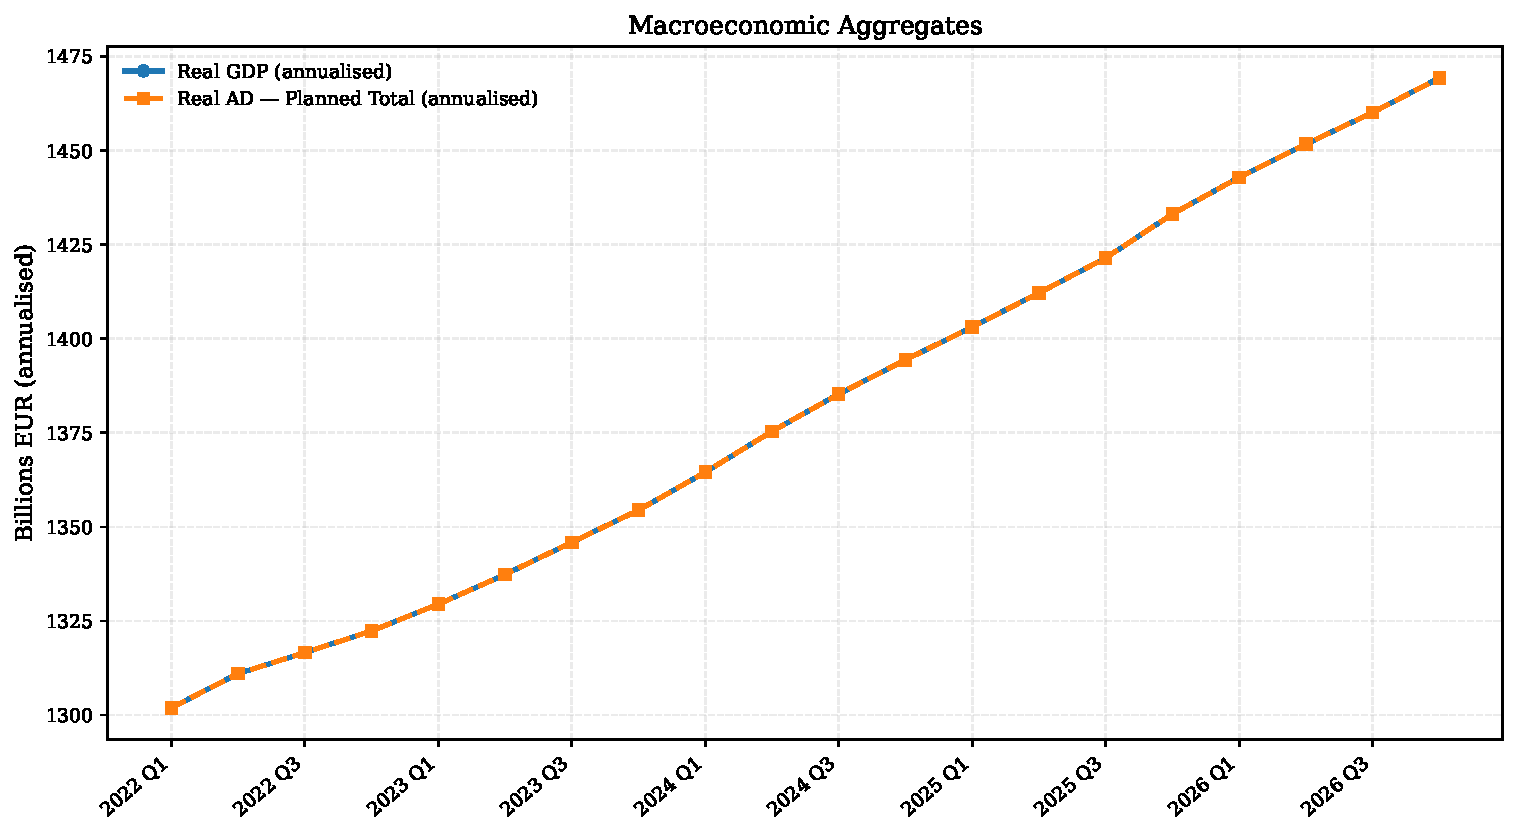
\includegraphics[width=\columnwidth]{figures/01_gdp.pdf}
    \caption{Comparison of simulated GDP against aggregate demand
             over 20 quarters.}
    \label{fig:gdpad}
\end{figure}

\paragraph{Bilateral transaction verification.}
This misreporting incentive can be neutralised through a double-entry recording
architecture in which every inter-firm transaction is registered bilaterally.
Firm $j$'s claim that it used $A_{ij} X_j$ units of good $i$ as an intermediate
input is automatically cross-checked against firm $i$'s record of the corresponding
output shipment. Any discrepancy between the buyer's input receipt and the
seller's delivery record is immediately flagged, making misreporting
self-revealing without requiring centralised auditing. This is structurally
analogous to value-added tax invoice matching, in which fiscal authorities
cross-reference purchase and sales invoices across firms to detect underreporting \citep{Pomeranz2015}. Applied to the planning context, the same
bilateral structure transforms the $A$ matrix from a self-reported document into
a verified accounting identity: the entry $A_{ij}$ is not what firm $j$ claims
to have used, but what firm $i$ and firm $j$ jointly recorded as transferred.
The aggregate material balance~\eqref{eq:material_balance} then holds by
construction at every planning period rather than as a statistical approximation.


\paragraph{Capital stock verification.}
Flow-based entries in $A$ are naturally bilateral and therefore self-verifying
under the double-entry architecture. Capital stock entries in $B$ are more
difficult to verify since a firm's held capital has no natural transaction
counterparty to cross-check against. One approach is indirect inference:
given observed gross output $\vec{X}_t$ and the material balance, the implied
capital requirement $\vec{K}_t = B\vec{X}_t$ can be computed centrally and
compared against firm reports. Persistent deviations between implied and
reported capital stocks provide a signal of either misreporting or genuine
technological change in the capital coefficient. Distinguishing between the
two requires either periodic physical audits or a Kalman-filter-style state
estimator that separates trend drift in $B$ from reporting noise, which we
leave as a direction for future work.